\documentclass[../main-physics-problems.tex]{subfiles}
\begin{document}

\subsection{Location and How Far}
\subsubsection{Position, Displacement, and Distance}

\begin{questions}

\begin{EnvUplevel}
    \textbf{Questions \ref{tex2J}--\ref{nOEef}.} Combine each of the 2 vectors graphically and mathematically.
\end{EnvUplevel} 

\question \label{tex2J}
10 meters East and 2 meters East

\question
\SI{14}{m} East and \SI{9}{m} West

\question
\SI{3}{m} up and \SI{5}{m} down

\question 
$+\SI{6}{m/s}$ and $-\SI{10}{m/s}$

\question
\SI{3}{m} North and \SI{4}{m} East

\question \label{nOEef}
\SI{6}{m} South and \SI{8}{m} West


\clearpage
\begin{EnvUplevel}
    \subsection{Distance and Displacement}   

    \textbf{Questions \ref{vyEPS}--\ref{m9Sn1}. With paper and ruler, measure the distance traveled and the displacement from the origin.}      
\end{EnvUplevel}

\clearpage

\question \label{vyEPS}
Station 1

\begin{center}
    \begin{tikzpicture}
        \draw[->, ultra thick] (0,0) node[below] {start} -- (0,11);
        \draw[->, ultra thick] (0,11) -- (7,11) node[right] {end};
    \end{tikzpicture}
\end{center}

\begin{solution}
\begin{center}
    \begin{tikzpicture}
        \draw[->, ultra thick] (0,0) node[below] {start} -- (0,11) node[left,pos=0.5] {11\,cm};
        \draw[->, ultra thick] (0,11) -- (7,11) node[above,pos=0.5] {7\,cm} node[right] {end};
        \draw[->, ultra thick, dashed] (0,0) -- (7,11) node[below right,pos=0.5] {13\,cm};
    \end{tikzpicture}
\end{center}

    \begin{align*}
        \text{distance} &= \SI{11}{cm} + \SI{7}{cm} = \SI{14}{cm}\\[1ex]
        \text{displacement} &= \SI{13}{cm}
    \end{align*}
\end{solution}



\clearpage

\question 
Station 2

\begin{center}
    \begin{tikzpicture}
        \draw[->, ultra thick] (0,0) node[left] {start} -- (6,0);
        \draw[->, ultra thick] (6,0) -- (6,4);
        \draw[->, ultra thick] (6,4) -- (9,4);
        \draw[->, ultra thick] (9,4) -- (9,11);
        \draw[->, ultra thick] (9,11) -- (7,11) node[above] {end};
        %\draw[->,ultra thick, dashed] (0,0) -- (7,11);
    \end{tikzpicture}
\end{center}

\begin{solution}
\begin{center}
    \begin{tikzpicture}
        \draw[->, ultra thick] (0,0) node[left] {start} -- (6,0) node[below,pos=0.5] {6\,cm};
        \draw[->, ultra thick] (6,0) -- (6,4) node[left,pos=0.5] {4\,cm};
        \draw[->, ultra thick] (6,4) -- (9,4) node[above,pos=0.5] {3\,cm};
        \draw[->, ultra thick] (9,4) -- (9,11) node[left,pos=0.5] {7\,cm};
        \draw[->, ultra thick] (9,11) -- (7,11) node[below,pos=0.5] {2\,cm} node[above] {end};
        \draw[->,ultra thick, dashed] (0,0) -- (7,11) node[above left, pos=0.5] {13\,cm};
    \end{tikzpicture}
\end{center}

    \begin{align*}
        \text{distance} &= \SI{6}{cm} + \SI{4}{cm} + \SI{3}{cm} + \SI{7}{cm} + \SI{2}{cm} = \SI{22}{cm}\\[1ex]
        \text{displacement} &= \SI{13}{cm}
    \end{align*}
\end{solution}



\clearpage
\question 
Station 3

\begin{center}
    \begin{tikzpicture}
        \draw[->, ultra thick] (0,0) node[left] {start} -- (5,0);
        \draw[->, ultra thick] (5,0) -- (5,-12);
        \draw[->, ultra thick] (5,-12) -- (0,-12) node[left] {end};
    \end{tikzpicture}
\end{center}

\begin{solution}
\begin{center}
    \begin{tikzpicture}
        \draw[->, ultra thick] (0,0) node[left] {start} -- (5,0) node[above,pos=0.5] {5\,cm};
        \draw[->, ultra thick] (5,0) -- (5,-12) node[right,pos=0.5] {12\,cm};
        \draw[->, ultra thick] (5,-12) -- (0,-12) node[below,pos=0.5] {5\,cm} node[left] {end};
        \draw[->,ultra thick,dashed] (0,0) -- (0,-12) node[left,pos=0.5] {12\,cm};
    \end{tikzpicture}
\end{center}

    \begin{align*}
        \text{distance} &= \SI{5}{cm} + \SI{12}{cm} + \SI{5}{cm}  = \SI{22}{cm}\\[1ex]
        \text{displacement} &= \SI{12}{cm}\ \text{down}
    \end{align*}
\end{solution}

\clearpage

\question \label{m9Sn1}
Station 4

\begin{center}
    \begin{tikzpicture}
        \draw[->, ultra thick] (0,0) node[left] {start} -- (7,0);
        \draw[->, ultra thick] (7,0) -- (7,-6);
        \draw[->, ultra thick] (7,-6) -- (5,-6);
        \draw[->, ultra thick] (5,-6) -- (5,-13) node[below] {end};
    \end{tikzpicture}
\end{center}

\begin{solution}
\begin{center}
    \begin{tikzpicture}
        \draw[->, ultra thick] (0,0) node[left] {start} -- (7,0) node[above,pos=0.5] {7\,cm};
        \draw[->, ultra thick] (7,0) -- (7,-6) node[right,pos=0.5] {6\,cm};
        \draw[->, ultra thick] (7,-6) -- (5,-6) node[above,pos=0.5] {2\,cm};
        \draw[->, ultra thick] (5,-6) -- (5,-13) node[right,pos=0.5] {7\,cm} node[below] {end};
        \draw[->, ultra thick, dashed] (0,0) -- (5,-13) node[left,pos=0.5] {14\,cm};
    \end{tikzpicture}
\end{center}


\end{solution}


\clearpage

\begin{center}
    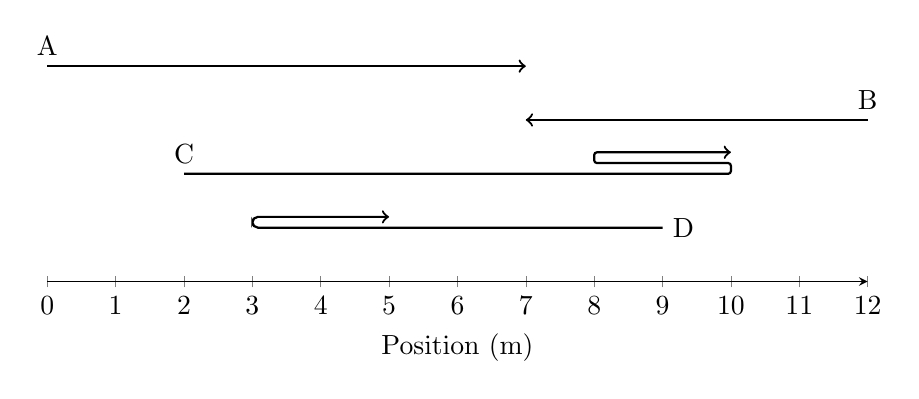
\begin{tikzpicture}
    \begin{axis}[width=12cm,height=5cm,
        axis lines = left,
        axis y line=none,
        xlabel = {Position (m)},
        ymin=0, ymax=5, 
        xmin=0, xmax=12,
        xtick={0,1,...,12},
        clip=false,
        ]
        \draw[->,thick] (0,4) node[above] {A} -- ++(7,0) ;
        \draw[->,thick] (12,3) node[above] {B} -- ++(-5,0) ;
        \draw[->,rounded corners=1pt,thick] (2,2) node[above] {C} -- ++(8,0) -- ++(0,0.2) -- ++(-2,0) -- ++(0,0.2) -- ++(2,0);
        \draw[->,rounded corners=2pt,thick] (9,1) node[right] {D} -- ++(-6,0) -- ++(0,0.2) -- ++(2,0);
    \end{axis}
    \end{tikzpicture}
\end{center}


\question \label{openstax-2.1}
Find the following for path A in the figure: 

\begin{parts}
    \part The distance traveled.

    \begin{solution}
        7\,m
    \end{solution}

    \part The displacement from start to finish.

    \begin{solution}
        7\,m
    \end{solution}
    
    \part The magnitude of the displacement.

    \begin{solution}
        7\,m
    \end{solution}
    
\end{parts}


\question \label{openstax-2.2}
Find the following for path B in the figure: 

\begin{parts}
    \part The distance traveled.
    \begin{solution}
        5\,m
    \end{solution}
    
    \part The displacement from start to finish.

    \begin{solution}
        \begin{equation*}
            \Delta x = x - x_0 = \SI{7}{m} - \SI{12}{m} = \boxed{\SI{-5}{m}}
        \end{equation*}
    \end{solution}
    
    \part The magnitude of the displacement.

    \begin{solution}
        \begin{equation*}
            \left|\Delta x\right| = \left|-\SI{5}{m}\right| = \boxed{\SI{5}{m}}
        \end{equation*}
    \end{solution}
\end{parts}


\question \label{openstax-2.3}
Find the following for path C in the figure: 

\begin{parts}
    \part The distance traveled.

    \begin{solution}
        \begin{equation*}
            D = \SI{8}{m} + \SI{2}{m} + \SI{2}{m} = \SI{12}{m}
        \end{equation*}
    \end{solution}
    
    \part The displacement from start to finish.

    \begin{solution}
        \begin{equation*}
            \Delta x = x - x_0 = \SI{10}{m} - \SI{2}{m} = \boxed{\SI{8}{m}}
        \end{equation*}
        
    \end{solution}
    \part The magnitude of the displacement.

    \begin{solution}
        8\,m
    \end{solution}
\end{parts}


\question \label{openstax-2.4}
Find the following for path D in the figure: 

\begin{parts}
    \part The distance traveled.
    \begin{solution}
        \begin{equation*}
            D = \SI{6}{m} + \SI{2}{m} = \SI{8}{m}
        \end{equation*}
    \end{solution}
    
    \part The displacement from start to finish.

    \begin{solution}
        \begin{equation*}
            \Delta x = x - x_0 = \SI{5}{m} - \SI{9}{m} = \boxed{-\SI{4}{m}}
        \end{equation*}
    \end{solution}
    
    \part The magnitude of the displacement.

    \begin{solution}
        \begin{equation*}
            \left|\Delta x\right| = \left|-\SI{4}{m}\right| = \boxed{\SI{4}{m}}
        \end{equation*}
    \end{solution}
    
\end{parts}

\clearpage
\begin{EnvUplevel}
    \subsection{Distance and Displacement (Part II)}
\end{EnvUplevel}

\question
Justin Credible runs the following route in 15 seconds: 50 meters in the negative direction, 30 meters in the positive direction, 15 meters in the negative direction, 40 meters in the positive direction, and 20 meters in the negative direction. 

\begin{parts}
\part What is the distance Justin ran?

\begin{solution}
    \begin{equation*}
        \text{distance} = \SI{50}{m} + \SI{30}{m} + \SI{15}{m} + \SI{40}{m} + \SI{20}{m} = \boxed{\SI{155}{m}}
    \end{equation*}
\end{solution}

\part What is Justin's displacement?

\begin{solution}
    \begin{equation*}
        \Delta x = \SI{-50}{m} + \SI{30}{m} - \SI{15}{m} + \SI{40}{m} - \SI{20}{m} = \boxed{\SI{-15}{m}}
    \end{equation*}
\end{solution}

\part What is his average speed?

\begin{solution}
    \begin{equation*}
        \text{speed} = \frac{\text{distance}}{\text{time}} = \boxed{\SI{10.3}{m/s}}
    \end{equation*}
\end{solution}

\part What is his average velocity?

\begin{solution}
    \begin{equation*}
        v = \frac{\Delta x}{\Delta t} = \boxed{\SI{-1}{m/s}}
    \end{equation*}
\end{solution}
\end{parts}

\question
A bus travels 280\,km south for 3.2 hours, stops for a lunch break for 0.4 hours, then travels 210\,km south for 2.8 hours. What is the average velocity for the total trip (in km/hr)?

\begin{solution}
    Using South as the negative direction, the displacement is
    
    \begin{equation*}
        \Delta x = -\SI{280}{km} - \SI{210}{km} = \SI{-490}{km}
    \end{equation*}

    The total time of travel is

    \begin{equation*}
        \Delta t = \SI{3.2}{h} + \SI{0.4}{h} + \SI{2.8}{h} = \SI{6.4}{h}
    \end{equation*}

    Therefore, average velocity is

    \begin{equation*}
        v = \frac{\Delta x}{\Delta t} = \boxed{\SI{-76.6}{km/h}}
    \end{equation*}
\end{solution}

\clearpage
\begin{EnvUplevel}
    \subsection{Position vs. Time Graphs}
\end{EnvUplevel}

\question
Consider the following motion graph.

\begin{center}
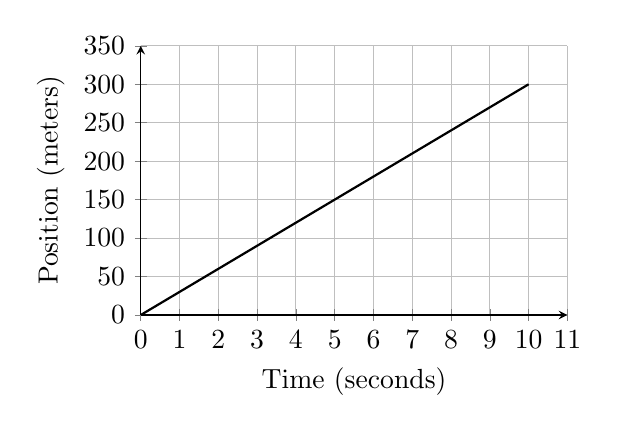
\begin{tikzpicture}
    \begin{axis}[height=5cm,
        width=7cm,
        axis lines=left,
        ylabel={Position (meters)},
        xlabel={Time (seconds)},
        ymin=0,ymax=350,
        xmin=0,xmax=11,
        ytick={0,50,...,350},
        xtick={0,1,...,11},
        grid=both,
    ]
        \addplot[thick,domain=0:10] {30*x};
    \end{axis}
\end{tikzpicture}
\end{center}

\begin{parts}
\part 
When did the object reach 150 meters?

\part 
Where was the object at 9 seconds?

\part
Find the slope of the graph. Show all your work.

\begin{solution}
\begin{center}
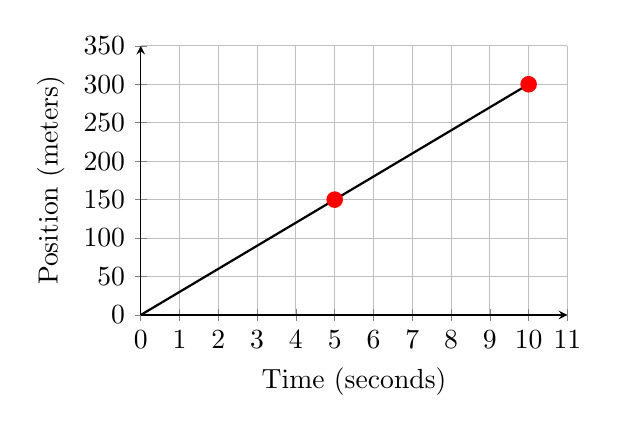
\begin{tikzpicture}
    \begin{axis}[height=5cm,
        width=7cm,
        axis lines=left,
        ylabel={Position (meters)},
        xlabel={Time (seconds)},
        ymin=0,ymax=350,
        xmin=0,xmax=11,
        ytick={0,50,...,350},
        xtick={0,1,...,11},
        grid=both,
    ]
        \addplot[thick,domain=0:10] {30*x};
        \fill[red] (5,150) circle (3pt);
        \fill[red] (10,300) circle (3pt);
    \end{axis}
\end{tikzpicture}
\end{center}

Using the two coordinates shown above, the slope is rise over run:

\begin{equation*}
    \text{slope} = \frac{\SI{300}{m} - \SI{150}{m}}{\SI{10}{s} - \SI{5}{s}} = \boxed{\SI{30}{m/s}}
\end{equation*}
\end{solution}


\part 
What physical quantity does the slope represent?


\end{parts}


\question
Consider the following motion graph.

\begin{center}
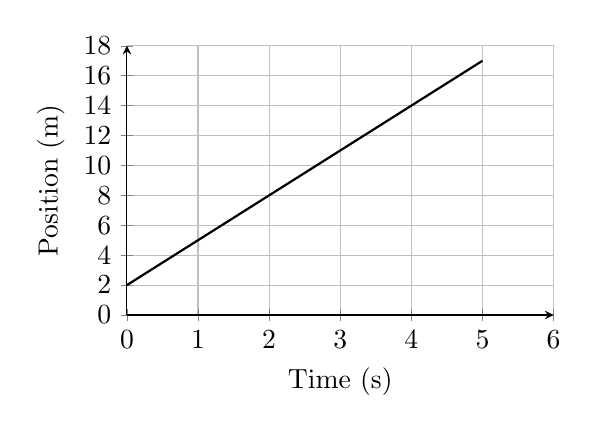
\begin{tikzpicture}
    \begin{axis}[height=5cm,
        width=7cm,
        axis lines=left,
        ylabel={Position (m)},
        xlabel={Time (s)},
        ymin=0,ymax=18,
        xmin=0,xmax=6,
        ytick={0,2,...,18},
        xtick={0,1,...,6},
        grid=both,
    ]
        \addplot[thick,domain=0:5] {3*x+2};
    \end{axis}
\end{tikzpicture}
\end{center}

\begin{parts}
\part 
Which is the independent variable?

\begin{solution}
    Time
\end{solution}

\part 
Which is the dependent variable?

\begin{solution}
    Position
\end{solution}

\part
Where was the object at 4 seconds?

\begin{solution}
    \SI{14}{m}
\end{solution}

\part
Find the slope of the graph. Show all your work.

\begin{solution}
\begin{center}
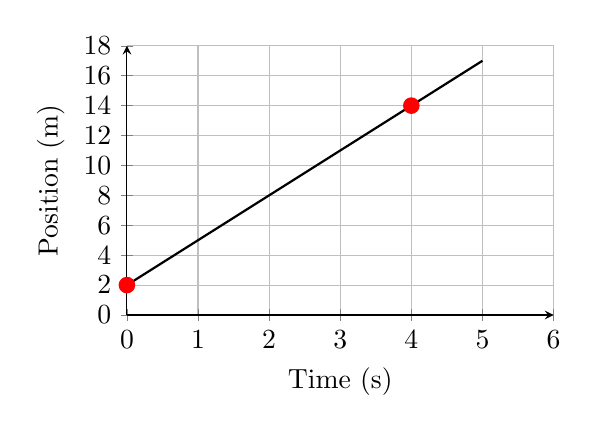
\begin{tikzpicture}
    \begin{axis}[height=5cm,
        width=7cm,
        axis lines=left,
        ylabel={Position (m)},
        xlabel={Time (s)},
        ymin=0,ymax=18,
        xmin=0,xmax=6,
        ytick={0,2,...,18},
        xtick={0,1,...,6},
        grid=both,
        clip=false,
    ]
        \addplot[thick,domain=0:5] {3*x+2};
        \fill[red] (0,2) circle (3pt);
        \fill[red] (4,14) circle (3pt);
    \end{axis}
\end{tikzpicture}
\end{center}

Using the two coordinates shown above, the slope is rise over run:

\begin{equation*}
    \text{slope} = \frac{\SI{14}{m} - \SI{2}{m}}{\SI{4}{s} - \SI{0}{s}} = \boxed{\SI{3}{m/s}}
\end{equation*}
\end{solution}


\part 
What physical quantity does the slope represent?


\end{parts}



\question 
Consider the position vs. time graph below. 

\begin{center}
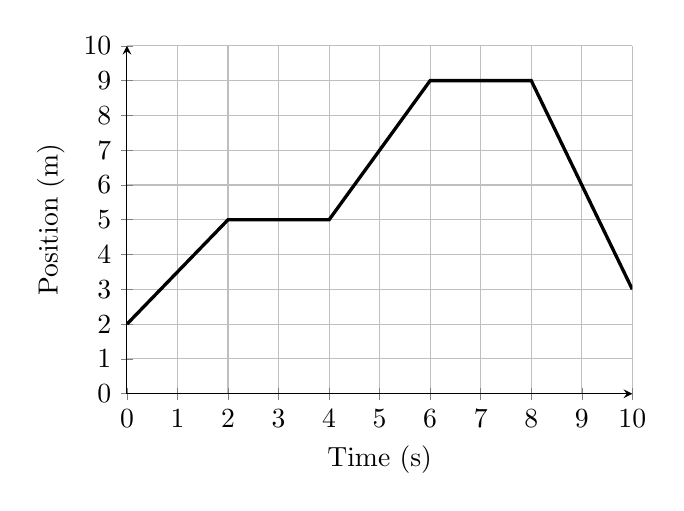
\begin{tikzpicture}
    \begin{axis}[width=8cm,height=6cm,
        axis lines=left,
        ymin=0, ymax=10,
        xmin=0, xmax=10,
        ylabel = {Position (m)},
        xlabel = {Time (s)},
        grid = both,
        xtick={0,1,...,10},
        ytick={0,1,...,10},
    ]
    \addplot[black,very thick]
        coordinates{(0,2)(2,5)(4,5)(6,9)(8,9)(10,3)};
\end{axis}
\end{tikzpicture}
\end{center}

\begin{parts}
\part How far did the object move between 0 and 2 seconds?

\begin{solution}
    The object moves 2 meters, since $\SI{5}{m} - \SI{3}{m} = \SI{2}{m}$.
\end{solution}


\part What happens from 2\,s to 4\,s?

\begin{solution}
    It stayed still. That is, it was not moving.
\end{solution}

\part At what time did it change direction?

\begin{solution}
    At 8 seconds.
\end{solution}

\part During what time interval was it moving fastest?

\begin{solution}
    From 8 seconds to the end.
\end{solution}

\part What is the object's velocity at $t = \SI{5}{s}$?

\begin{solution}
    Velocity is the slope of the line: \SI{2}{m/s}.
\end{solution}
\end{parts}

\question
Look at the following position vs. time graph.

\begin{center}
    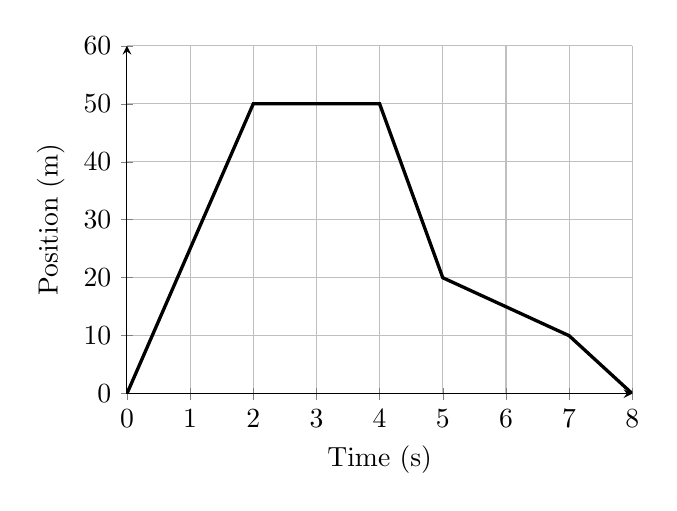
\begin{tikzpicture}
        \begin{axis}[width=8cm,height=6cm,
            ymin=0,ymax=60,
            xmin=0,xmax=8,
            axis lines=left,
            ylabel={Position (m)},
            xlabel={Time (s)},
            grid=both,
            ytick={0,10,...,60},
            xtick={0,1,...,8},
        ]
            \addplot[black,very thick]
                coordinates{(0,0)(2,50)(4,50)(5,20)(7,10)(8,0)};
        \end{axis}
    \end{tikzpicture}
\end{center}

\begin{parts}
\part What was the initial position of the
object?

\begin{solution}
    0 meters
\end{solution}

\part What was the object’s position at 3s?

\begin{solution}
    50 meters
\end{solution}

\part At about what time did the object reach 30\,m?

\begin{solution}
    Between 4 and 5 seconds (about 4.5 seconds).
\end{solution}

\part When did the object turn around?

\begin{solution}
    4 seconds.
\end{solution}
\end{parts}

\clearpage
\begin{EnvUplevel}
    \subsection{Dune Buggy Lab (Part I)}
\end{EnvUplevel}




\question
The teacher demonstrates the first trial of the lab. Here's some sample data.

\begin{minipage}{0.45\textwidth}
    \centering
    \begin{tabular}{c|c}
        \hline
        Time (s) & Position (m) \\ \hline
        2.3 & 0 \\
        5.0 & 1 \\
        7.6 & 2 \\
        9.9 & 3 \\
        12.4 & 4 \\
        14.9 & 5 \\
        17.5 & 6 \\
         19.9 & 7 \\
         22.5 & 8 \\
    \end{tabular}
\end{minipage}%
\hspace{1em}
\begin{minipage}{0.45\textwidth}
    \centering
    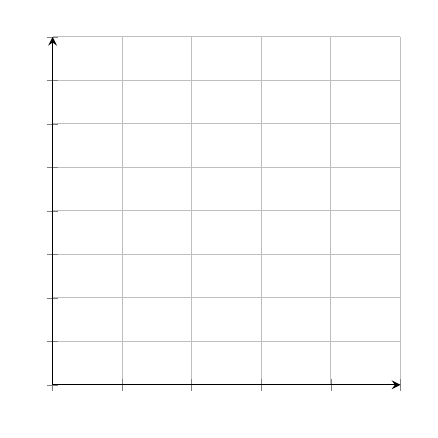
\begin{tikzpicture}
        \begin{axis}[height=6cm,width=6cm,
            % ylabel={Position (m)},
            % xlabel={Time (s)},
            ymin=0,ymax=8,
            xmin=0,xmax=25,
            ytick={0,1,...,8},
            xtick={0,5,...,25},
            xticklabels=\empty,
            yticklabels=\empty,
            axis lines=left,
            grid=both,
        ]
        %\addplot[mark=*,only marks] coordinates{(2.3,0)(5.0,1)(7.6,2)(9.9,3)(12.4,4)(14.9,5)(17.5,6)(19.9,7)(22.5,8)};
        \end{axis}
    \end{tikzpicture}
\end{minipage}

Student's do the following parts:

\begin{parts}
    \part Make a graph for position vs. time for the buggy. Then draw a best-fit-line of the data. Label the axes with correct quantities and units.

\begin{solution}
\phantom{.}

\begin{minipage}{0.45\textwidth}
    \centering
    \begin{tabular}{c|c}
        \hline
        Time (s) & Position (m) \\ \hline
        2.3 & 0 \\
        5.0 & 1 \\
        7.6 & 2 \\
        9.9 & 3 \\
        12.4 & 4 \\
        14.9 & 5 \\
        17.5 & 6 \\
         19.9 & 7 \\
         22.5 & 8 \\
    \end{tabular}
\end{minipage}%
\hspace{1em}
\begin{minipage}{0.45\textwidth}
    \centering
    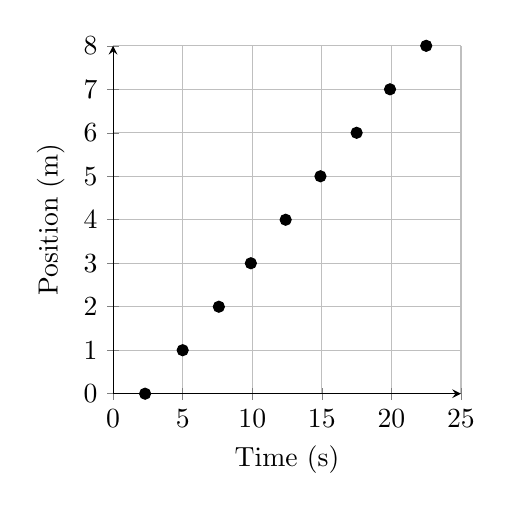
\begin{tikzpicture}
        \begin{axis}[height=6cm,width=6cm,
            ylabel={Position (m)},
            xlabel={Time (s)},
            ymin=0,ymax=8,
            xmin=0,xmax=25,
            ytick={0,1,...,8},
            xtick={0,5,...,25},
            axis lines=left,
            grid=both,
        ]
        \addplot[mark=*,only marks] coordinates{(2.3,0)(5.0,1)(7.6,2)(9.9,3)(12.4,4)(14.9,5)(17.5,6)(19.9,7)(22.5,8)};
        \end{axis}
    \end{tikzpicture}
\end{minipage}

\end{solution}

    \part Calculate the slope of the line, with the correct units. (Answers may vary.)

\begin{solution}
    To find slope, choose any two points and compute rise (change in position) over run (change in time). For example, choosing coordinates

    \begin{equation*}
        (\text{time\,1},\text{pos\,1}) = (\SI{7.6}{s},\SI{2}{m}) \qquad \text{and} \qquad
        (\text{time\,2},\text{pos\,2}) = (\SI{17.5}{s},\SI{6}{m})
    \end{equation*}
    
    the slope is

    \begin{equation*}
        \text{slope} = \frac{\text{pos\,2} - \text{pos\,1}}{\text{time\,2} - \text{time\,1}} 
        = \frac{\SI{6}{m} - \SI{2}{m}}{\SI{17.5}{s} - \SI{7.6}{s}} = \boxed{\SI{0.404}{m/s}}
    \end{equation*}

    \bigskip

    On a calculator, use parentheses like this:

    \medskip

    \begin{center}
        \texttt{(6-2)/(17.5-7.6)}\\
        \hspace{2.5em} \texttt{.404040404}
    \end{center}
\end{solution}

\end{parts}

% \vspace{5mm}

% \begin{minipage}{0.45\textwidth}
%     \centering
%     \begin{tabular}{c|c}
%         \hline
%         Time (s) & Position (m) \\ \hline
%         2.68 & 0 \\
%         5.14 & 1 \\
%         7.16 & 2 \\
%         10.03 & 3 \\
%         12.13 & 4 \\
%         14.80 & 5 \\
%         17.05 & 6 \\
%         19.67 & 7 \\
%         21.72 & 8 \\
%     \end{tabular}
% \end{minipage}%
% \hspace{1em}
% \begin{minipage}{0.45\textwidth}
%     \centering
%     \begin{tikzpicture}
%         \begin{axis}[height=6cm,width=6cm,
%             ylabel={Position (m)},
%             xlabel={Time (s)},
%             ymin=0,ymax=8,
%             xmin=0,xmax=25,
%             ytick={0,1,...,8},
%             xtick={0,5,...,25},
%             axis lines=left,
%             grid=both,
%         ]
%         \addplot[mark=*,only marks] coordinates{(2.68,0)(5.14,1)(7.16,2)(10.03,3)(12.13,4)(14.8,5)(17.05,6)(19.67,7)(21.72,8)};
%         \end{axis}
%     \end{tikzpicture}
% \end{minipage}

\clearpage
\begin{EnvUplevel}
    \subsection{Dune Buggy Lab (Part II)}
\end{EnvUplevel}



\question
Warm-Up: Sketch a position vs. time graph for the following scenario:

A girl walks from the reference point forward to \SI{5}{m} in 3 seconds. Then she stops for about 2 seconds. Finally she walks back to the reference point over 5 seconds.

%Be ready to share your graph on your whiteboard

\begin{solution}
\begin{center}
    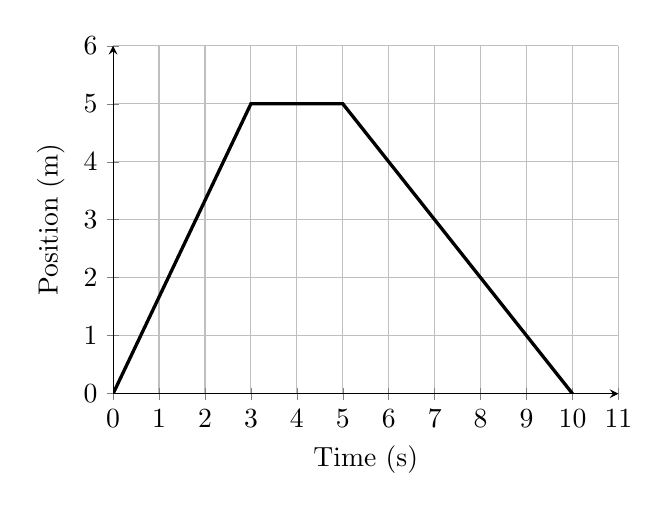
\begin{tikzpicture}
        \begin{axis}[width=8cm,height=6cm,
            ymin=0,ymax=6,
            xmin=0,xmax=11,
            axis lines=left,
            ylabel={Position (m)},
            xlabel={Time (s)},
            grid=both,
            ytick={0,1,...,6},
            xtick={0,1,...,11},
        ]
            \addplot[black,very thick]
                coordinates{(0,0)(3,5)(5,5)(10,0)};
        \end{axis}
    \end{tikzpicture}
\end{center}
\end{solution}


%...Source: teacher.desmos.com by Teagan Bourne. Transcribed into LaTeX.
\question
Consider the graph below. 

\begin{center}
    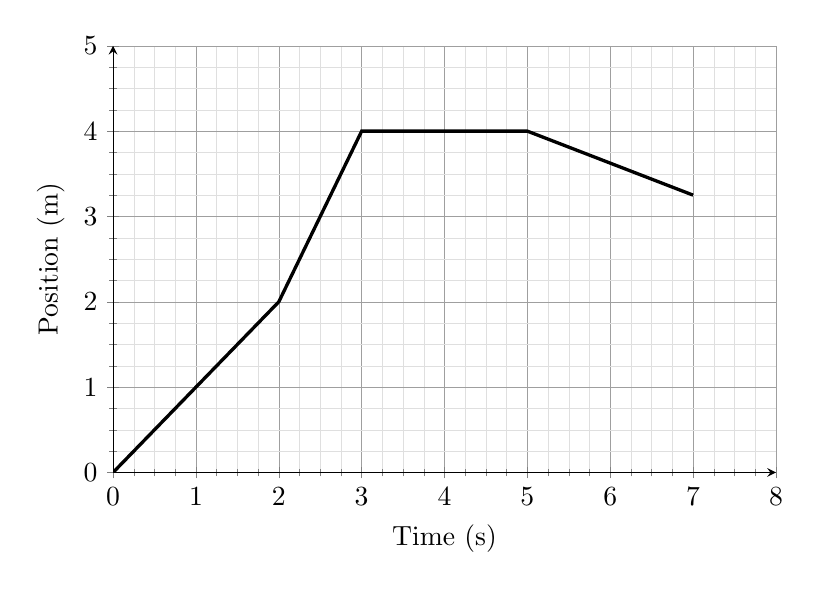
\begin{tikzpicture}
        \begin{axis}[width=10cm,height=7cm,
            ymin=0,ymax=5,
            xmin=0,xmax=8,
            axis lines=left,
            ylabel={Position (m)},
            xlabel={Time (s)},
            grid=both,
            ytick={0,1,...,5},
            xtick={0,1,...,8},
            minor tick num=3,
            minor grid style={line width=.2pt,draw=gray!25},
            major grid style={line width=.2pt,draw=gray!75},
        ]
            \addplot[black,very thick]
                coordinates{(0,0)(2,2)(3,4)(5,4)(7,3.25)};
        \end{axis}
    \end{tikzpicture}
\end{center}

\begin{parts}
\part What is the distance traveled by the object between 2 and 3 seconds as seen in this graph?

\begin{solution}
    2 meters.
\end{solution}

\part What is the distance traveled by the object between 2 and 5 seconds as seen in this graph?

\begin{solution}
    2 meters.
\end{solution}

\part What is the total distance traveled by the object as seen in this graph?

\begin{solution}
    4.75 meters.
\end{solution}

\part
What is the total displacement of the object as seen in this graph?

\begin{solution}
    3.25 meters
\end{solution}
\end{parts}

\question
Consider the next graph.

\begin{center}
    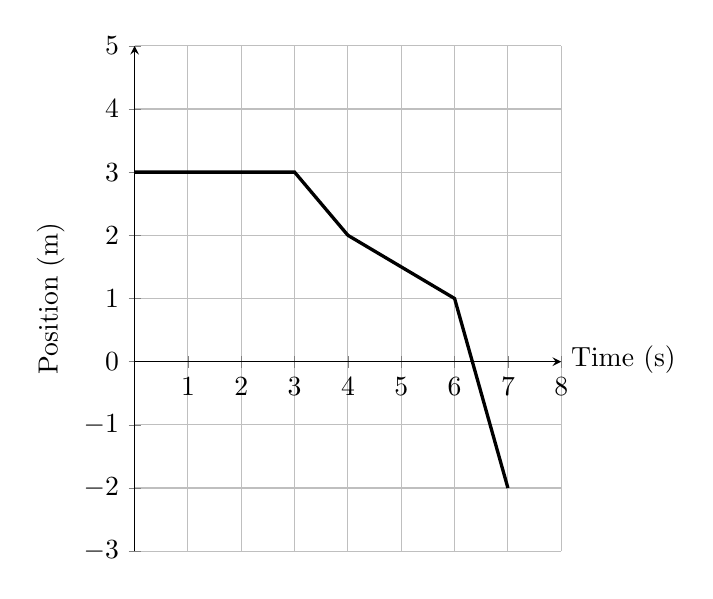
\begin{tikzpicture}
        \begin{axis}[width=7cm,height=8cm,
            ymin=-3,ymax=5,
            xmin=0,xmax=8,
            axis y line=left,
            axis x line = center,
            ylabel={Position (m)},
            xlabel={Time (s)},
            grid=both,
            ytick={-3,-2,...,5},
            xtick={0,1,...,8},
            x label style={at={(axis description cs:1,0.38)},anchor=west},
        ]
            \addplot[black,very thick]
                coordinates{(0,3)(3,3)(4,2)(6,1)(7,-2)};
        \end{axis}
    \end{tikzpicture}
\end{center}

\begin{parts}
\part What is the distance traveled by the object between 1 and 3 seconds as seen in this graph?

\begin{solution}
    0 meters. The object did not move.
\end{solution}

\part
Which time is the beginning of the fastest motion of the object?

\begin{solution}
    6 seconds.
\end{solution}

\part What is the total distance traveled by the object as seen in this graph?

\begin{solution}
    5 meters
\end{solution}

\part What is the total displacement of the object as seen in this graph?

\begin{solution}
    \SI{-5}{m} or 5 meters in the negative direction.
\end{solution}
\end{parts}

\question
Consider this graph.

\begin{center}
    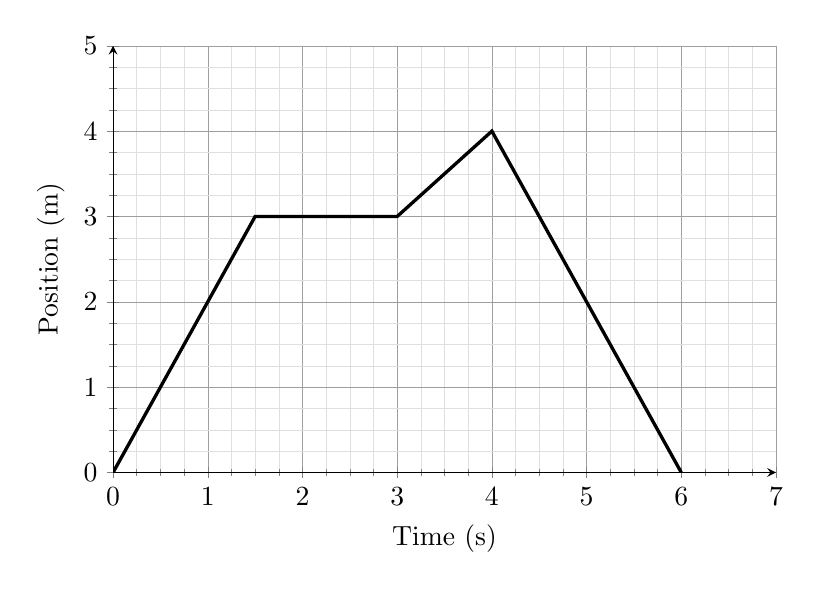
\begin{tikzpicture}
        \begin{axis}[width=10cm,height=7cm,
            ymin=0,ymax=5,
            xmin=0,xmax=7,
            axis lines=left,
            ylabel={Position (m)},
            xlabel={Time (s)},
            grid=both,
            ytick={0,1,...,5},
            xtick={0,1,...,7},
            minor tick num=3,
            minor grid style={line width=.2pt,draw=gray!25},
            major grid style={line width=.2pt,draw=gray!75},
        ]
            \addplot[black,very thick]
                coordinates{(0,0)(1.5,3)(3,3)(4,4)(6,0)};
        \end{axis}
    \end{tikzpicture}
\end{center}

\begin{parts}
\part What is the total distance traveled by the object as seen in this graph?

\begin{solution}
    8 meters
\end{solution}

\part What is the total displacement of the object as seen in this graph?

\begin{solution}
    0 meters
\end{solution}
\end{parts}



\clearpage

\begin{EnvUplevel}
    \subsection{Speed and Velocity}
\end{EnvUplevel}


\question 
Exit Ticket: Convert the position vs time graph to a velocity vs time graph.

\begin{center}
    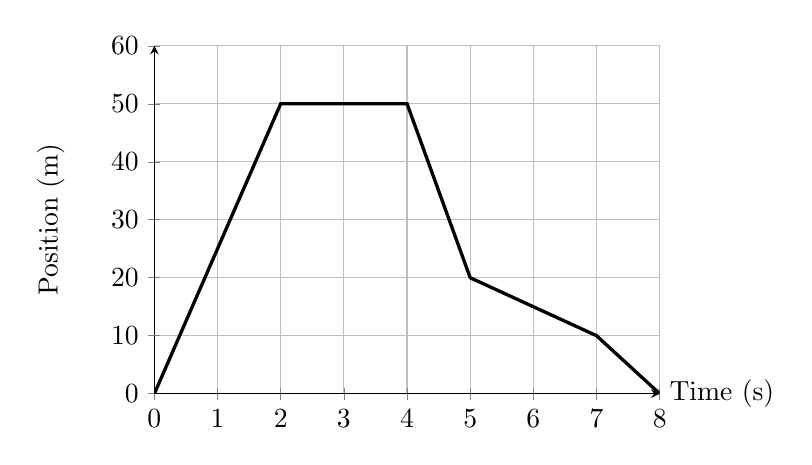
\begin{tikzpicture}
        \begin{axis}[width=8cm,height=6cm,
            ymin=0,ymax=60,
            xmin=0,xmax=8,
            axis lines=left,
            ylabel={Position (m)},
            xlabel={Time (s)},
            grid=both,
            ytick={0,10,...,60},
            xtick={0,1,...,8},
            extra y ticks={10},
            extra y tick style={yticklabel=\phantom{$-10$}},
            x label style={at={(axis description cs:1,0)},anchor=west},
        ]
            \addplot[black,very thick]
                coordinates{(0,0)(2,50)(4,50)(5,20)(7,10)(8,0)};
        \end{axis}
    \end{tikzpicture}

    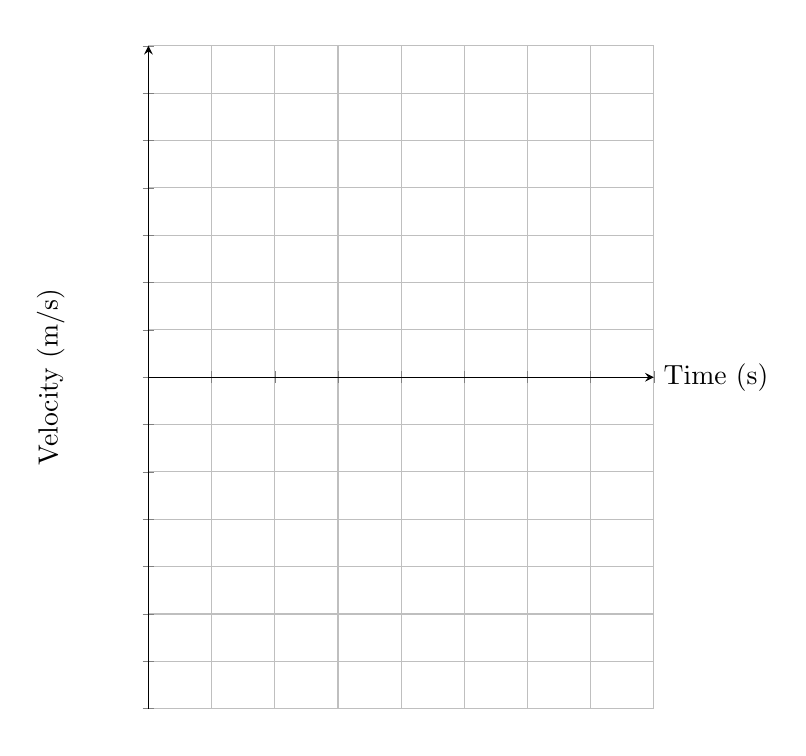
\begin{tikzpicture}
        \begin{axis}[width=8cm,height=10cm,
            axis y line=left,
            axis x line=center,
            ylabel={Velocity (m/s)},
            xlabel={Time (s)},
            ymin=-35,ymax=35,
            xmin=0,xmax=8,
            grid=both,
            ytick={-35,-30,...,35},
            xtick={0,1,...,8},
            xticklabel=\empty,
            x label style={at={(axis description cs:1,0.5)},anchor=west},
            yticklabel style={white},
        ]
        \end{axis}
    \end{tikzpicture}
\end{center}

\begin{solution}
\begin{center}
    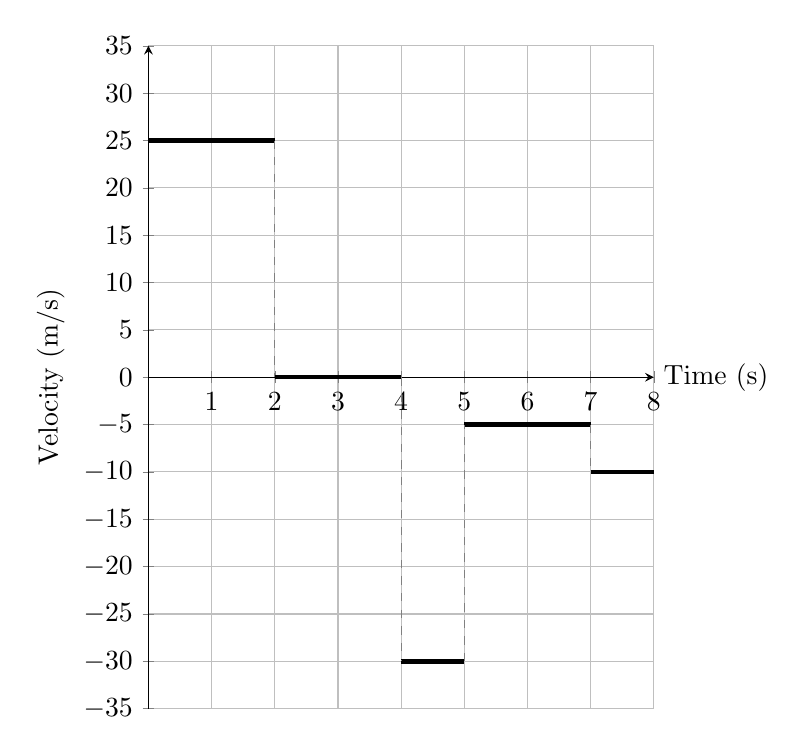
\begin{tikzpicture}
        \begin{axis}[width=8cm,height=10cm,
            axis y line=left,
            axis x line=center,
            ylabel={Velocity (m/s)},
            xlabel={Time (s)},
            ymin=-35,ymax=35,
            xmin=0,xmax=8,
            grid=both,
            ytick={-35,-30,...,35},
            xtick={0,1,...,8},
            x label style={at={(axis description cs:1,0.5)},anchor=west},
        ]
        %\addplot[black,ultra thick] coordinates{(0,25)(2,25)(2,0)(4,0)(4,-30)(5,-30)(5,-5)(7,-5)(7,-10)(8,-10)};
        \addplot[black,ultra thick] coordinates {(0,25)(2,25)};
        \addplot[black,ultra thick] coordinates {(2,0)(4,0)};
        \addplot[black,ultra thick] coordinates {(4,-30)(5,-30)};
        \addplot[black,ultra thick] coordinates {(5,-5)(7,-5)};
        \addplot[black,ultra thick] coordinates {(7,-10)(8,-10)};
        \addplot[gray,dashed] coordinates {(2,25)(2,0)};
        \addplot[gray,dashed] coordinates {(4,0)(4,-30)};
        \addplot[gray,dashed] coordinates {(5,-30)(5,-5)};
        \addplot[gray,dashed] coordinates {(7,-5)(7,-10)};
        \end{axis}
    \end{tikzpicture}
\end{center}
\end{solution}

\clearpage
\begin{EnvUplevel}
\subsection{Speed and Velocity (Part II)}

    \textbf{Questions \ref{WC4WJ}--\ref{qjQqH}.} For the questions below, draw the corresponding graph.
\end{EnvUplevel}

\question \label{WC4WJ}
Given the position vs time graph, draw the corresponding velocity vs time graph.

\begin{center}
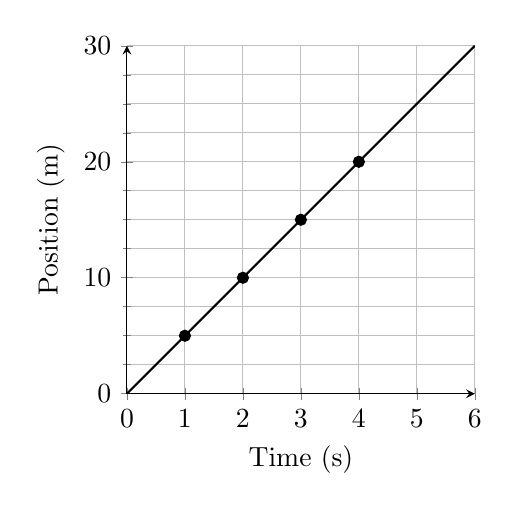
\begin{tikzpicture}
    \begin{axis}[width=6cm,height=6cm,
        ymin=0,ymax=30,
        xmin=0,xmax=6,
        axis lines=left,
        ylabel={Position (m)},
        xlabel={Time (s)},
        grid=both,
        ytick={0,10,...,30},
        xtick={0,1,...,6},
        minor y tick num=3,
        grid=both
    ]
        \addplot[black,thick,]
            coordinates{(0,0)(6,30)};
        \addplot[black,mark=*]
            coordinates{(1,5)(2,10)(3,15)(4,20)};
    \end{axis}
\end{tikzpicture}%
\hspace{1cm}
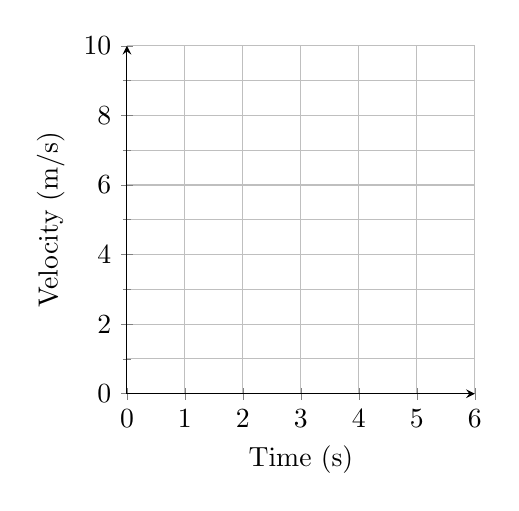
\begin{tikzpicture}
    \begin{axis}[width=6cm,height=6cm,
        ymin=0,ymax=10,
        xmin=0,xmax=6,
        axis lines=left,
        ylabel={Velocity (m/s)},
        xlabel={Time (s)},
        grid=both,
        ytick={0,2,...,10},
        xtick={0,1,...,6},
        minor y tick num=1,
        grid=both
    ]
    \end{axis}
\end{tikzpicture}

\bigskip

\hspace{8cm}
\begin{tabular}{|c|c|}
    \hline
    \textbf{time} (s) & \textbf{velocity} (m/s) \\ \hline
     & \\ \hline
     & \\ \hline
     & \\ \hline
     & \\ \hline
\end{tabular}
\end{center}

\question
Next graphs:

\begin{center}
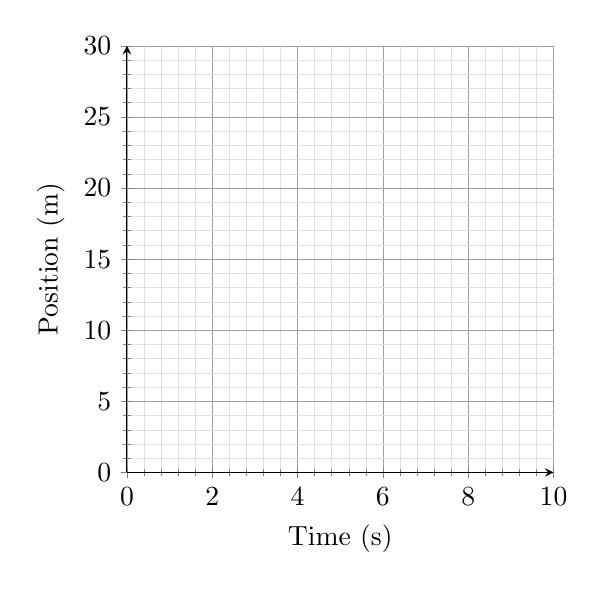
\begin{tikzpicture}
    \begin{axis}[width=7cm,height=7cm,
        ymin=0,ymax=30,
        xmin=0,xmax=10,
        axis lines=left,
        ylabel={Position (m)},
        xlabel={Time (s)},
        grid=both,
        ytick={0,5,...,30},
        xtick={0,2,...,10},
        minor tick num=4,
        grid=both,
        minor grid style={line width=.2pt,draw=gray!25},
        major grid style={line width=.2pt,draw=gray!75},
    ]
    %\addplot[black,ultra thick,domain=0:20]{3*x};
    \end{axis}
\end{tikzpicture}%
\hspace{1cm}
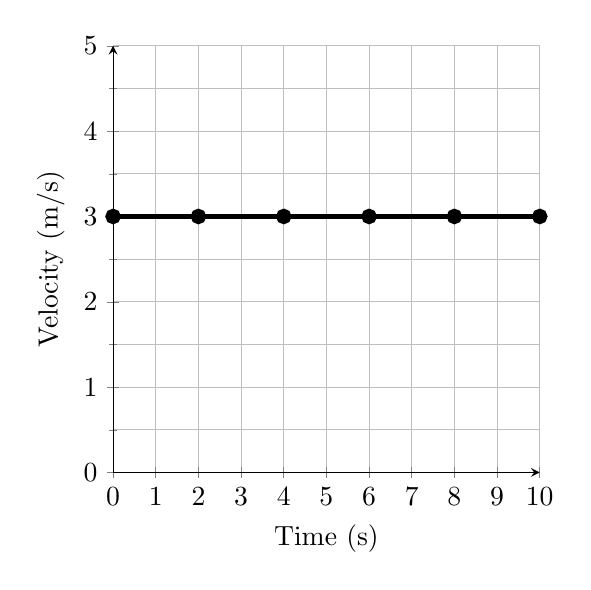
\begin{tikzpicture}
    \begin{axis}[width=7cm,height=7cm,
        ymin=0,ymax=5,
        xmin=0,xmax=10,
        axis lines=left,
        ylabel={Velocity (m/s)},
        xlabel={Time (s)},
        grid=both,
        ytick={0,1,...,5},
        xtick={0,1,...,10},
        minor y tick num=1,
        grid=both
    ]
    \addplot[black,ultra thick,mark=*] coordinates{(0,3)(2,3)(4,3)(6,3)(8,3)(10,3)};
    \end{axis}
\end{tikzpicture}
\end{center}

\begin{solution}
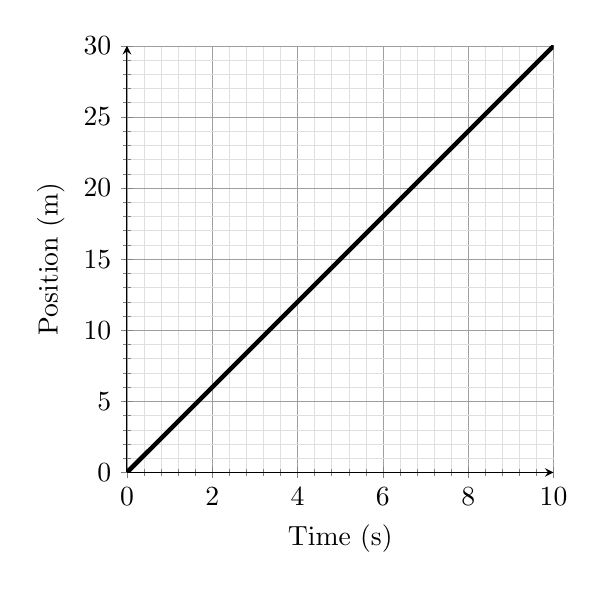
\begin{tikzpicture}
    \begin{axis}[width=7cm,height=7cm,
        ymin=0,ymax=30,
        xmin=0,xmax=10,
        axis lines=left,
        ylabel={Position (m)},
        xlabel={Time (s)},
        grid=both,
        ytick={0,5,...,30},
        xtick={0,2,...,10},
        minor tick num=4,
        grid=both,
        minor grid style={line width=.2pt,draw=gray!25},
        major grid style={line width=.2pt,draw=gray!75},
    ]
    \addplot[black,ultra thick,domain=0:20]{3*x};
    \end{axis}
\end{tikzpicture}
\end{solution}

\question
An object starts at the reference point and moves with a constant velocity of 10\,m/s for 3\,s. Draw the position vs time and velocity vs time graphs.

\begin{solution}
\begin{center}
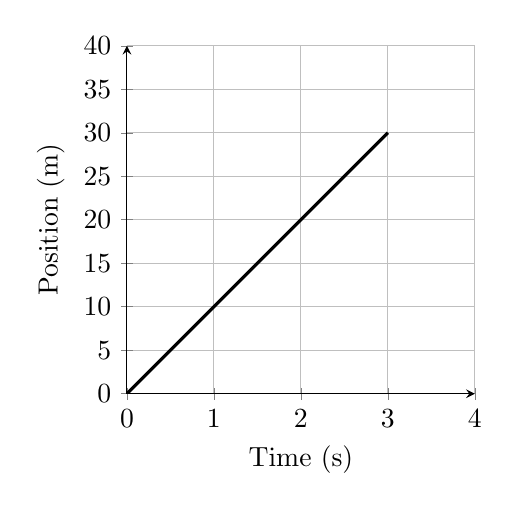
\begin{tikzpicture}
    \begin{axis}[width=6cm,height=6cm,
        ymin=0,ymax=40,
        xmin=0,xmax=4,
        axis lines=left,
        ylabel={Position (m)},
        xlabel={Time (s)},
        grid=both,
        ytick={0,5,...,40},
        xtick={0,1,...,4},
        grid=both
    ]
    \addplot[black,very thick,domain=0:3]{10*x};
    \end{axis}
\end{tikzpicture}%
\hspace{5mm}
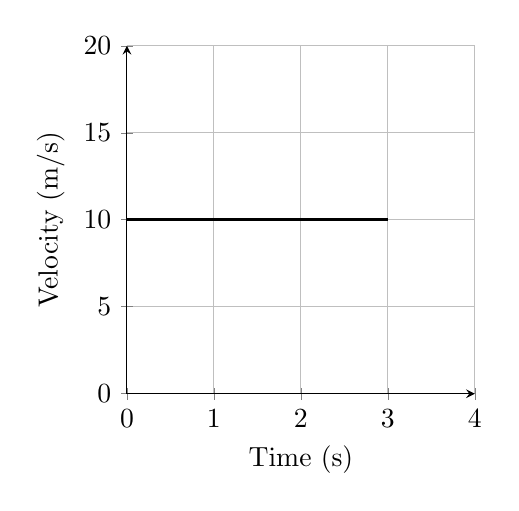
\begin{tikzpicture}
    \begin{axis}[width=6cm,height=6cm,
        ymin=0,ymax=20,
        xmin=0,xmax=4,
        axis lines=left,
        ylabel={Velocity (m/s)},
        xlabel={Time (s)},
        grid=both,
        ytick={0,5,...,20},
        xtick={0,1,...,4},
        %minor y tick num=1,
        grid=both
    ]
    \addplot[black,very thick,domain=0:3] {10};
    \end{axis}
\end{tikzpicture}
\end{center}
\end{solution}

\question
The table below describes the motion of an object:

\begin{center}
    \begin{tabular}{|c|c|}
        \hline
        $x$ (m) & $t$ (s) \\ \hline
         0 & 0 \\ \hline
         1 & 2 \\ \hline
         2 & 4 \\ \hline
         3 & 6 \\ \hline
    \end{tabular}
\end{center}

Graph the object's position and velocity as functions of time.

\begin{solution}
\begin{center}
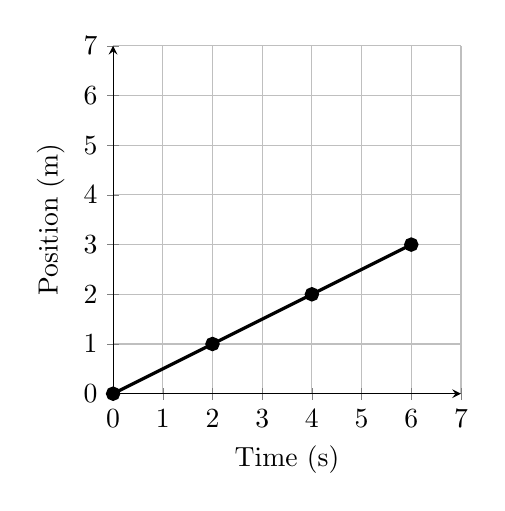
\begin{tikzpicture}
    \begin{axis}[width=6cm,height=6cm,
        ymin=0,ymax=7,
        xmin=0,xmax=7,
        axis lines=left,
        ylabel={Position (m)},
        xlabel={Time (s)},
        grid=both,
        ytick={0,1,...,7},
        xtick={0,1,...,7},
        grid=both
    ]
    \addplot[black,very thick,mark=*] coordinates{(0,0)(2,1)(4,2)(6,3)};
    \end{axis}
\end{tikzpicture}%
\hspace{5mm}
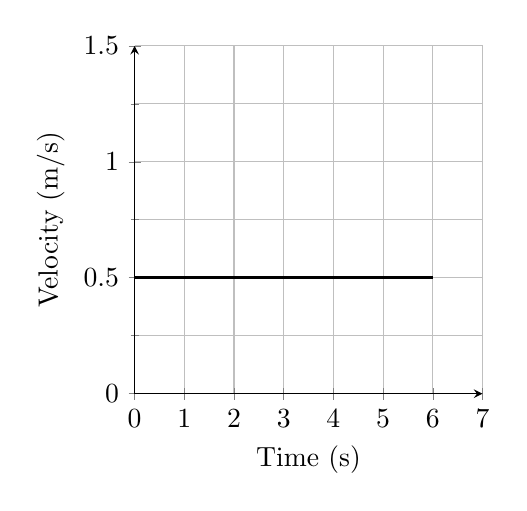
\begin{tikzpicture}
    \begin{axis}[width=6cm,height=6cm,
        ymin=0,ymax=1.5,
        xmin=0,xmax=7,
        axis lines=left,
        ylabel={Velocity (m/s)},
        xlabel={Time (s)},
        grid=both,
        ytick={0,0.5,...,1.5},
        xtick={0,1,...,7},
        minor y tick num=1,
        grid=both
    ]
    \addplot[black,very thick,domain=0:6] {0.5};
    \end{axis}
\end{tikzpicture}
\end{center}
\end{solution}

\question
Object moves with constant positive velocity for 4 seconds. Then, it stops for 2 seconds and returns to the initial position in 2 seconds.

\begin{solution}
Student graphs will vary due to choice of velocity.

\begin{center}
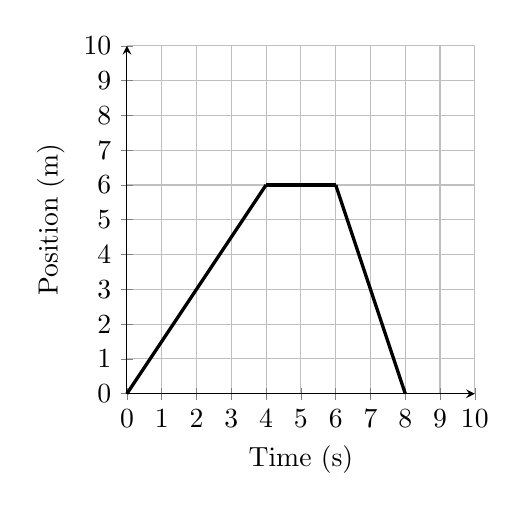
\begin{tikzpicture}
    \begin{axis}[width=6cm,height=6cm,
        ymin=0,ymax=10,
        xmin=0,xmax=10,
        axis lines=left,
        ylabel={Position (m)},
        xlabel={Time (s)},
        grid=both,
        ytick={0,1,...,10},
        xtick={0,1,...,10},
        grid=both,
        clip=false
    ]
    \addplot[black,very thick,domain=0:4]{3/2*x};
    \addplot[black,very thick,domain=4:6]{6};
    \addplot[black,very thick,domain=6:8]{-3*(x-6)+6};
    \end{axis}
\end{tikzpicture}%
\hspace{5mm}
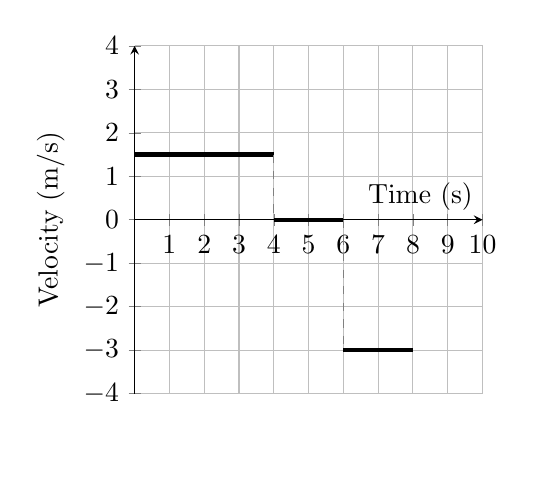
\begin{tikzpicture}
    \begin{axis}[width=6cm,height=6cm,
        ymin=-4,ymax=4,
        xmin=0,xmax=10,
        axis y line=left,
        axis x line=center,
        ylabel={Velocity (m/s)},
        xlabel={Time (s)},
        grid=both,
        ytick={-4,-3,...,4},
        xtick={0,1,...,10},
        grid=both,
        clip=false,
    ]
    \addplot[black,ultra thick,domain=0:4] {3/2};
    \addplot[black,ultra thick,domain=4:6] {0};
    \addplot[black,ultra thick,domain=6:8] {-3};
    \addplot[gray,dashed] coordinates{(4,1.5)(4,0)};
    \addplot[gray,dashed] coordinates{(6,0)(6,-3)};
    \node at (0,-5) {\phantom{Time (s)}};
    \end{axis}
\end{tikzpicture}
\end{center}
\end{solution}

\question
Draw the velocity vs. time graph that corresponds to the graph below.

\begin{center}
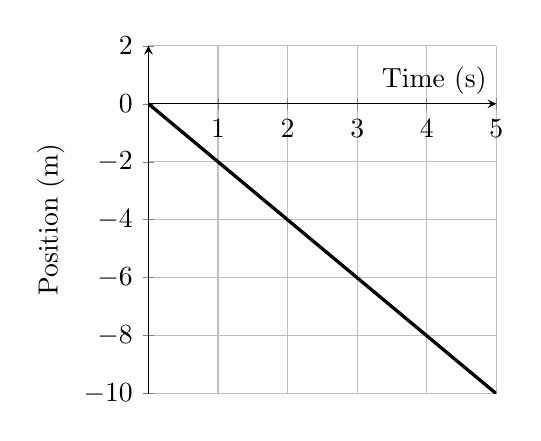
\begin{tikzpicture}
    \begin{axis}[width=6cm,height=6cm,
        ymin=-10,ymax=2,
        xmin=0,xmax=5,
        axis y line=left,
        axis x line=center,
        ylabel={Position (m)},
        xlabel={Time (s)},
        grid=both,
        ytick={2,0,...,-10},
        xtick={0,1,...,5},
        grid=both
    ]
    \addplot[black,very thick,domain=0:5]{-2*x};
    \end{axis}
\end{tikzpicture}    
\end{center}

\begin{solution}
\begin{center}
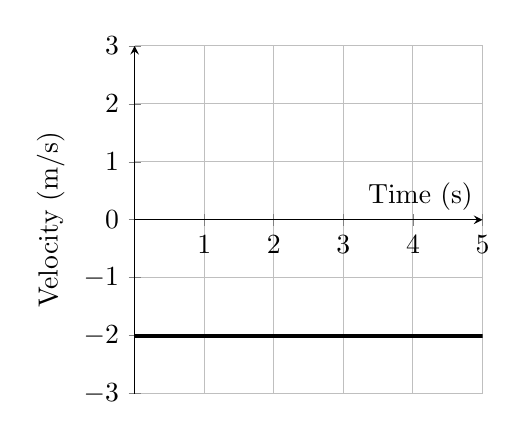
\begin{tikzpicture}
    \begin{axis}[width=6cm,height=6cm,
        ymin=-3,ymax=3,
        xmin=0,xmax=5,
        axis y line=left,
        axis x line=center,
        ylabel={Velocity (m/s)},
        xlabel={Time (s)},
        grid=both,
        ytick={-3,-2,...,3},
        xtick={0,1,...,5},
        grid=both
    ]
    \addplot[black,ultra thick,domain=0:5] {-2};
    \end{axis}
\end{tikzpicture}
\end{center}
\end{solution}

\question
An object's motion is summarized in the table below. Graph positive vs time and velocity vs time when the object's initial position is $x_i = \SI{50}{m}$.

\begin{center}
\begin{tabular}{|c|c|}
    \hline
    $t$ (s) & $v$ (m/s) \\ \hline
     0 & 100 \\ \hline
     1 & 100 \\ \hline
     2 & 100 \\ \hline
\end{tabular}
\end{center}

\begin{solution}
\begin{center}
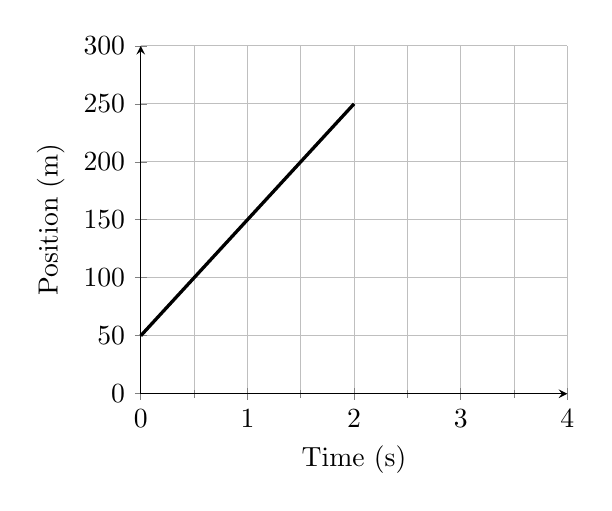
\begin{tikzpicture}
    \begin{axis}[width=7cm,height=6cm,
        ymin=0,ymax=300,
        xmin=0,xmax=4,
        axis lines=left,
        ylabel={Position (m)},
        xlabel={Time (s)},
        grid=both,
        ytick={0,50,...,300},
        xtick={0,1,...,4},
        minor x tick num=1,
        grid=both,
        clip=false
    ]
    \addplot[black,very thick,domain=0:2]{100*x+50};
    \end{axis}
\end{tikzpicture}%
\hspace{5mm}
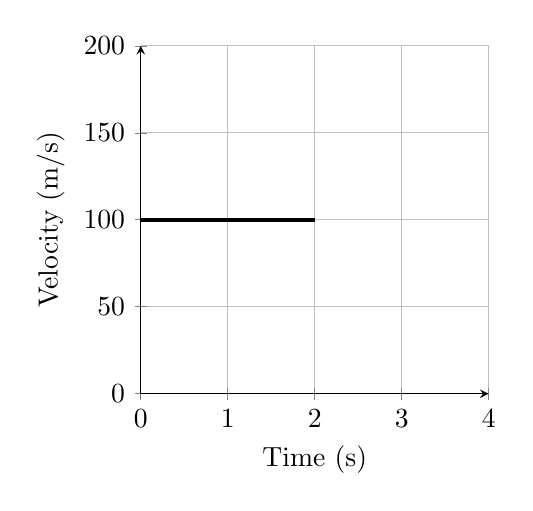
\begin{tikzpicture}
    \begin{axis}[width=6cm,height=6cm,
        ymin=0,ymax=200,
        xmin=0,xmax=4,
        axis lines = left,
        ylabel={Velocity (m/s)},
        xlabel={Time (s)},
        grid=both,
        ytick={0,50,...,200},
        xtick={0,1,...,4},
        grid=both,
    ]
    \addplot[black,ultra thick,domain=0:2] {100};
    \end{axis}
\end{tikzpicture}
\end{center}    
\end{solution}

\question
Object A starts 10\,m to the right of the origin and moves to the left at 2\,m/s for 5\,s.

Object B starts at the origin and moves to the right at 3\,m/s.

\begin{solution}
\begin{center}
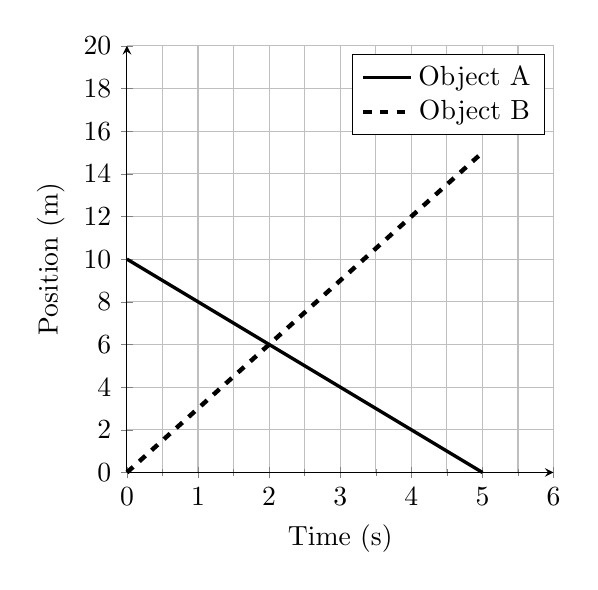
\begin{tikzpicture}
    \begin{axis}[width=7cm,height=7cm,
        ymin=0,ymax=20,
        xmin=0,xmax=6,
        axis lines=left,
        ylabel={Position (m)},
        xlabel={Time (s)},
        grid=both,
        ytick={0,2,...,20},
        xtick={0,1,...,6},
        minor x tick num=1,
        % minor y tick num=4,
        grid=both,
        clip=false
    ]
    \addplot[black,very thick,domain=0:5]{-2*x+10};
    \addlegendentry{Object A}
    \addplot[black,ultra thick,dashed,domain=0:5]{3*x};
    \addlegendentry{Object B}
    \end{axis}
\end{tikzpicture}%
\hspace{5mm}
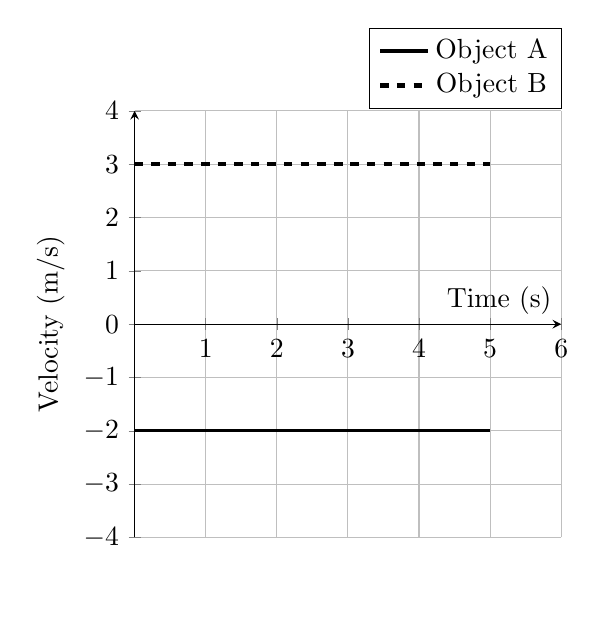
\begin{tikzpicture}
    \begin{axis}[width=7cm,height=7cm,
        ymin=-4,ymax=4,
        xmin=0,xmax=6,
        axis y line = left,
        axis x line = center,
        ylabel={Velocity (m/s)},
        xlabel={Time (s)},
        grid=both,
        ytick={-4,-3,...,4},
        xtick={0,1,...,6},
        grid=both,
        clip=false,
        legend style={at={(0.55,1.1)},anchor=west}
    ]
    \addplot[black,very thick,domain=0:5] {-2};
    \addlegendentry{Object A}
    \addplot[black,ultra thick,dashed,domain=0:5] {3};
    \addlegendentry{Object B}
    \node at (0,-5) {\phantom{Hello World}};
    \end{axis}
\end{tikzpicture}
\end{center}
\end{solution}

\question \label{qjQqH}
Consider this graph.

\begin{center}
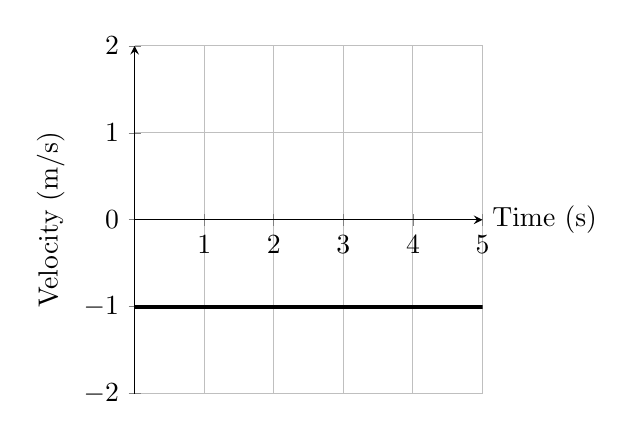
\begin{tikzpicture}
    \begin{axis}[width=6cm,height=6cm,
        ymin=-2,ymax=2,
        xmin=0,xmax=5,
        axis y line=left,
        axis x line=center,
        ylabel={Velocity (m/s)},
        xlabel={Time (s)},
        grid=both,
        ytick={-2,-1,...,2},
        xtick={0,1,...,5},
        grid=both,
        x label style={at={(axis description cs: 1,0.5)},anchor=west},
    ]
    \addplot[black,ultra thick,domain=0:5] {-1};
    \end{axis}
\end{tikzpicture}
\end{center}

Draw the corresponding position vs time graph.

\begin{solution}
\begin{center}
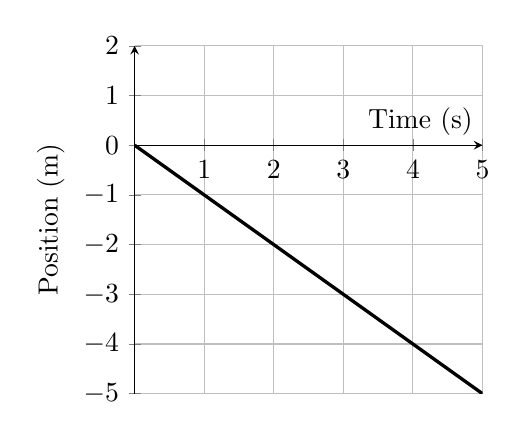
\begin{tikzpicture}
    \begin{axis}[width=6cm,height=6cm,
        ymin=-5,ymax=2,
        xmin=0,xmax=5,
        axis y line=left,
        axis x line=center,
        ylabel={Position (m)},
        xlabel={Time (s)},
        grid=both,
        ytick={2,1,...,-5},
        xtick={0,1,...,5},
        grid=both
    ]
    \addplot[black,very thick,domain=0:5]{-x};
    \end{axis}
\end{tikzpicture}    
\end{center}    
\end{solution}

\question 
Exit Ticket: A ball is thrown straight upward and falls back to the same height. A student makes this graph of the velocity of the ball as a function of time. 

\begin{center}
    \begin{tikzpicture}
        \draw[->] (0,0) -- (0.0,3) node[above] {$v$ (m/s)};
        \draw[->] (0,0) -- (3.5,0) node[right] {$t$ (s)};
        \draw[very thick] (0,2) -- (1.5,0) -- (3,2);
    \end{tikzpicture}
\end{center}

Work with your table to write what is wrong with the graph and how they should fix it on your whiteboard.

\begin{solution}
    The above graph shows the velocity always being positive or zero, implying the ball is always moving upwards, which is not what actually happens. In reality, after the ball reaches peak height, it's velocity will become negative:

    \begin{center}
        \begin{tikzpicture}
            \draw[->] (0,-2) -- (0.0,3) node[above] {$v$ (m/s)};
            \draw[->] (0,0) -- (3.5,0) node[right] {$t$ (s)};
            \draw[very thick] (0,2) -- (3,-2);
        \end{tikzpicture}
    \end{center}    
\end{solution}

\clearpage
\begin{EnvUplevel}
    \subsection{Mass and Inertia}
\end{EnvUplevel}

\question
Which has more inertia, a mouse or an elephant? Why?

\begin{solution}
    An elephant has more inertia because it has more mass than a mouse.
\end{solution}

\question
Rank the objects from least to most inertia:

Object A: $v = \SI{2}{m/s}$ and $m = \SI{10}{kg}$\\
Object B: $v = \SI{0}{m/s}$ and $m = \SI{20}{kg}$\\
Object C: $v = \SI{4}{m/s}$ and $m = \SI{5}{kg}$\\
Object D: $v = \SI{3}{m/s}$ and $m = \SI{8}{kg}$

\begin{solution}
    To rank by inertia, we rank them by increasing mass: C, D, A, B
\end{solution}

\question
If you were playing football would you rather be tackled by the kicker or a linebacker? Why?

\begin{solution}
    The kicker, he has less mass and inertia.
\end{solution}

\clearpage
\begin{EnvUplevel}
    \subsection{Momentum}
\end{EnvUplevel}

\question

A car possesses \SI[group-separator={,}]{20000}{kg\cdot m/s} of momentum. What would the momentum be if...

\begin{parts}
    \part its velocity was doubled?

    \begin{solution}
        $2 \times \SI[group-separator={,}]{20000}{kg\cdot m/s} = \boxed{\SI[group-separator={,}]{40000}{kg\cdot m/s}}$
    \end{solution}
    
    \part its mass were doubled?

    \begin{solution}
        $2 \times \SI[group-separator={,}]{20000}{kg \cdot m/s} = \boxed{\SI[group-separator={,}]{40000}{kg\cdot m/s}}$
    \end{solution}
    
    \part its velocity and mass were doubled?

    \begin{solution}
        $2 \times 2 \times \SI[group-separator={,}]{20000}{kg \cdot m/s} = \boxed{\SI[group-separator={,}]{80000}{kg\cdot m/s}}$
    \end{solution}
\end{parts}


\question 
A 10\,kg object with a velocity of 2\,m/s north will have how much momentum?

\begin{solution}
    \begin{align*}
        p &= mv\\[1ex]
          &= (\SI{10}{kg})(\SI{2}{m/s})\\[1ex]
          &= \boxed{\SI{20}{kg\cdot m/s}}
    \end{align*}
\end{solution}

\clearpage
\begin{EnvUplevel}
    \subsection{Kinetic Energy}
\end{EnvUplevel}

\question
What must be true for an object to have kinetic energy?

\begin{solution}
    The object must be in motion.
\end{solution}

\question 
Finish the following sentences:

\begin{parts}
    \part When speed increases, kinetic energy \fillin[increases].
    \part When speed decreases, kinetic energy \fillin[decreases].
    \part When an object stops it has \fillin[no] kinetic energy
\end{parts}

\question \label{taHSMX}
Dante, the 10-kilogram pitbull, runs with a velocity of 5.0 meters per second. What is Dante's kinetic energy?

\begin{solution}
\SI{125}{J}
\end{solution}

\question \label{QRI2H9}
What is the kinetic energy of a student of mass \SI{60}{kg} running at \SI{3.0}{m/s}?

\begin{solution}
\SI{270}{J}
\end{solution}


\question \label{ixc46e}
Sasha, the majestic eagle, flies in a straight line at \SI{20}{m/s}. What is the kinetic energy of the \SI{10}{kg} Sasha? 

\begin{solution}
\SI{2000}{J}
\end{solution}


\question \label{dguWEr}
(\textit{Try this problem by hand: no calculator.}) At a speed of \SI{10}{m/s}, a \SI{248}{kg} boulder hurls down the mountain. What is the boulder's kinetic energy?

\begin{solution}
\SI{12400}{J}
\end{solution}

\question \label{rUr2P8}
Your school's fastest sprinter jogs with a kinetic energy of \SI{1620}{J}. If their mass is \SI{90}{kg}, how fast are they moving?

\begin{solution}
\SI{6.0}{m/s}
\end{solution}

\question \label{2rrR9W}
Niyjah Huston skates down the street with a kinetic energy and velocity of \SI{5400}{J} and \SI{12}{m/s}, respectively. What is Niyjah's mass?

\begin{solution}
\SI{75}{kg}
\end{solution}

\question \label{gHlhnM}
A \SI{100}{kg} object moves with \SI{7500}{J} of kinetic energy. Calculate the object's speed.

\begin{solution}
\ref{gHlhnM} \SI{12.2}{m/s}
\end{solution}


\question \label{WH6xot}
When a skate rides their board at a speed of \SI{5.76}{m/s}, their energy of motion is \SI{2008}{J}. Find the skater's mass.

\begin{solution}
\SI{121}{kg}
\end{solution}

\question \label{X7RPxf}
A \SI{1263}{kg} asteroid travels at \SI{67}{m/s} through empty space. What is the astroid's kinetic energy?

\begin{solution}
\SI{2.83e6}{J}
\end{solution}

\clearpage
\begin{EnvUplevel}
    \subsection{Momentum and Kinetic Energy}
\end{EnvUplevel}

\question %44
List at least 3 facts in each section of the Venn Diagram:

\begin{center}
    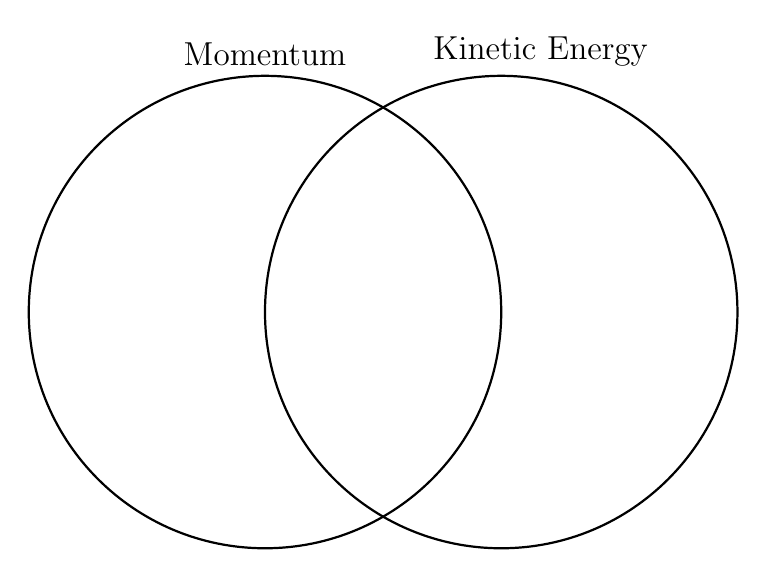
\begin{tikzpicture}
        \draw[thick] (0,0) circle (3cm) node[above=3cm] {\large Momentum};
        \begin{scope}[xshift=3cm]
            \draw[thick] (0,0) circle (3cm);
            \node[above] at (0.5,3) {\large Kinetic Energy};
        \end{scope}
    \end{tikzpicture}
\end{center}

\begin{solution}
\phantom{.}

Momentum:

\begin{itemize}[itemsep=0pt,topsep=0pt]
    \item $p=mv$
    \item units are \SI{}{kg\cdot m/s}
    \item proportional to velocity
\end{itemize}

\bigskip

Kinetic energy:

\begin{itemize}[itemsep=0pt,topsep=0pt]
    \item $\mathrm{KE} = \frac{1}{2} mv^2$
    \item unit is the joule (J) 
    \item proportional to velocity squared
\end{itemize}

\bigskip

both:

\begin{itemize}[itemsep=0pt,topsep=0pt]
    \item depend on mass and velocity
    \item are non-zero when the object is in motion
    \item increase when velocity increases
\end{itemize}
\end{solution}



\question %45
A 100\,kg man is running at 5.6\,m/s. What is his momentum? 

\begin{solution}
\phantom{.}

\begin{equation*}
    p = mv = \boxed{\SI{560}{kg\cdot m/s}}
\end{equation*}
\end{solution}



\question %47
An object has a kinetic energy of 25\,J and a mass of 34\,kg. How fast is the object moving? 

\begin{solution}
Solving the kinetic energy equation

\begin{equation*}
    \mathrm{KE} = \frac{1}{2} mv^2
\end{equation*}

for speed leads to

\begin{equation*}
    v = \sqrt{\frac{2\mathrm{KE}}{m}} = \boxed{\SI{1.21}{m/s}}
\end{equation*}
\end{solution}

\question %48
If a 40\,kg object has a momentum of \SI{400}{kg\cdot m/s}, how fast is it traveling?

\begin{solution}
Solving the momentum equation $p = mv$ for speed leads to

\begin{equation*}
    v = \frac{p}{m} = \boxed{\SI{10}{kg\cdot m/s}}
\end{equation*}
\end{solution}

% \question %49
% If you can run 15 miles per hour (6.7\,m/s) while holding a 8 pound (3.5\,kg) shot put, how much momentum does the shot put have?     

% \begin{solution}
%     \begin{equation*}
%         p = mv = \boxed{\SI{23.45}{kg\cdot m/s}}
%     \end{equation*}
% \end{solution}
     
\question %50
What is the kinetic energy of a 1200\,kg object that is moving with a speed of 24\,m/s? 

\begin{solution}
\begin{equation*}
    \mathrm{KE} = \frac{1}{2} mv^2 = \boxed{\SI{3.46e5}{J}}
\end{equation*}
\end{solution}

\question %51
A child running down the hall with a speed of 2.9\,m/s has a momentum of \SI{45.5}{kg\cdot m/s}. What is his mass?

\begin{solution}
Solving the momentum equation $p = mv$ for mass leads to 

\begin{equation*}
    m = \frac{p}{v} = \boxed{\SI{15.7}{kg}}
\end{equation*}
\end{solution}



% \question %53
% A truck travels 430\,m in 37\,s.  If its momentum is \SI[group-separator={,}]{91200}{kg\cdot m/s}, what is the mass of the truck? 

% \begin{solution}
% The truck's displacement is $\Delta x = \SI{430}{m}$, and the elapsed time is $\Delta t = \SI{37}{s}$. The truck's velocity is

% \begin{equation*}
%     v = \frac{\Delta x}{\Delta t} = \frac{\SI{430}{m}}{\SI{37}{s}} = \SI{11.6}{m/s}
% \end{equation*}

% So, solving the momentum equation $p = mv$ for mass leads to 

% \begin{equation*}
%     m = \frac{p}{v} = \frac{\SI[group-separator={,}]{91200}{kg\cdot m/s}}{\SI{11.6}{m/s}} = \boxed{\SI{7.8e3}{kg}}
% \end{equation*}

% \end{solution}

% \question %54
% Determine the momentum of a 360,000-kg passenger plane taxiing down a runway at 1.5\,m/s. 

% \begin{solution}
% \begin{equation*}
%     p = mv = \boxed{\SI{5.4e5}{kg\cdot m/s}}
% \end{equation*}
% \end{solution}



\question %56
A brown bear runs at with a velocity of 9.0\,m/s and a kinetic energy of 23,000\,J. What is the bear’s mass?

\begin{solution}
Solving the kinetic energy equation

\begin{equation*}
    \mathrm{KE} = \frac{1}{2} mv^2
\end{equation*}

for mass leads to

\begin{equation*}
    m = \frac{2\mathrm{KE}}{v^2} = \boxed{\SI{568}{kg}}
\end{equation*}
\end{solution}

% \question %57
% An airplane with a mass of 94,300\,kg flies 3960\,m in 561 seconds.  What is the momentum of the airplane?

% \begin{solution}
% The plane's velocity is

% \begin{equation*}
%     v = \frac{\Delta x}{\Delta t} = \frac{\SI{3960}{m}}{\SI{561}{s}} = \SI{7.06}{m/s}
% \end{equation*}

% The momentum is

% \begin{equation*}
%     p = mv = \boxed{\SI{6.7e5}{kg\cdot m/s}}
% \end{equation*}
% \end{solution}

% \question %58
% A toy car with a mas of 2.8\,kg has a momentum of \SI{150}{kg\cdot m/s}. How fast is it going?

% \begin{solution}
% Solving the momentum equation $p = mv$ for velocity leads to 

% \begin{equation*}
%     v = \frac{p}{m} = \boxed{\SI{53.6}{m/s}}
% \end{equation*}
% \end{solution}

\question %59
A basketball player with a mass of 91.7\,kg runs a distance of 98.2\,m in 55.9 seconds.  How much momentum does he have?

\begin{solution}
The player's displacement is

\begin{equation*}
    v = \frac{\Delta x}{\Delta t} = {\SI{1.76}{m/s}}
\end{equation*}

His momentum is therefore

\begin{equation*}
    p = mv = \boxed{\SI{161}{kg\cdot m/s}}
\end{equation*}
\end{solution}


% \question %61
% A cannon launches a 3.0\,kg pumpkin with 110\,J of kinetic energy. After 5 seconds, how far has the pumpkin moved?

% \begin{solution}
% Solving the kinetic energy equation 

% \begin{equation*}
%     \mathrm{KE} = \frac{1}{2} m v^2
% \end{equation*}

% for velocity leads to 

% \begin{equation*}
%     v = \sqrt{\frac{2\mathrm{KE}}{m}} = \SI{8.56}{m/s}
% \end{equation*}

% So, solving the velocity equation

% \begin{equation*}
%     v = \frac{\Delta x}{\Delta t}
% \end{equation*}

% for displacement leads to

% \begin{equation*}
%     \Delta x = v \Delta t = \boxed{\SI{42.8}{m}}
% \end{equation*}
% \end{solution}

% \question %62
% A stuffed toy with a mass of 0.3\,kg is thrown 4.2\,m across a room in such a way that it has a momentum of \SI{97}{kg\cdot m/s}.  How long did it take to cross the room? 

% \begin{solution}
% Solving the momentum equation $p = mv$ for velocity leads to

% \begin{equation*}
%     v = \frac{p}{m} = \SI{323}{m/s}
% \end{equation*}

% solving the velocity equation

% \begin{equation*}
%     v = \frac{\Delta x}{\Delta t}
% \end{equation*}

% for time leads to

% \begin{equation*}
%     \Delta t = \frac{\Delta x}{v} = \boxed{\SI{0.013}{s}}
% \end{equation*}
% \end{solution}

\question %46
What is the kinetic energy of a 150\,kg object that is moving with a speed of 15\,m/s? 

\begin{solution}
\phantom{.}

\begin{equation*}
    \mathrm{KE} = \frac{1}{2}mv^2 = \boxed{\SI{1.69e4}{J}}
\end{equation*}
\end{solution}

\question %52
An object has a kinetic energy of 14\,J and a mass of 17\,kg , how fast is the object moving? 

\begin{solution}
Solving the kinetic energy equation

\begin{equation*}
    \mathrm{KE} = \frac{1}{2} mv^2
\end{equation*}

for speed leads to

\begin{equation*}
    v = \sqrt{\frac{2\mathrm{KE}}{m}} = \boxed{\SI{1.28}{m/s}}
\end{equation*}
\end{solution}

\question %55
An elephant kicks a 5.0\,kg stone with 150\,J of kinetic energy. What is the velocity of the stone? 

\begin{solution}
Solving the kinetic energy equation

\begin{equation*}
    \mathrm{KE} = \frac{1}{2} mv^2
\end{equation*}

for speed leads to

\begin{equation*}
    v = \sqrt{\frac{2\mathrm{KE}}{m}} = \boxed{\SI{7.75}{m/s}}
\end{equation*}
\end{solution}

\question %60
A 30\,kg dog runs 45 meters in 3 seconds. What is the kinetic energy of the dog?

\begin{solution}
The velocity is

\begin{equation*}
    v = \frac{\Delta x}{\Delta t} = \frac{\SI{45}{m}}{\SI{3}{s}} = \SI{15}{m/s}
\end{equation*}

The kinetic energy is

\begin{equation*}
    \mathrm{KE} = \frac{1}{2} m v^2 = \boxed{\SI{3375}{J}}
\end{equation*}
\end{solution}




\question %64
An object has a kinetic energy of 88\,J and a mass of 45\,kg. How fast is the object moving?

\begin{solution}
Solving the kinetic energy equation 

\begin{equation*}
    \mathrm{KE} = \frac{1}{2}mv^2
\end{equation*}

for velocity leads to

\begin{equation*}
    v = \sqrt{\frac{2\mathrm{KE}}{m}} = \boxed{\SI{1.98}{m/s}}
\end{equation*}
\end{solution}
 
\question %65
Exit Ticket: Thomas and Maria are talking about which object has more momentum, a motorcycle going 50\,m/s or an 18-wheeler at a stoplight. 

Thomas says that the 18-wheeler must have more because it has more mass. 

Maria disagrees. Help her explain why Thomas is incorrect. Write at least 1 complete sentence.

\begin{solution}
    The 18-wheeler has a velocity of $v = 0$, and since momentum is $p = mv$, it has zero momentum. 
\end{solution}

\clearpage
\begin{EnvUplevel}
    \subsection{Relative Velocity}
\end{EnvUplevel}

\question
A group of friends riding home on the bus need your help solving an argument. They are looking at their backpacks sitting on the bus seats next to them and they each make a point. 

Gabriel: ``The bags aren't moving. Look at mine, it’s sitting right next to me!''

Hanna: ``The bags are moving as fast as we are because we are on the bus.''

Ali: ``The bags are moving even faster than we think! Millions of miles per hour because the whole Earth is moving!''

Decide who is right and explain why in at least two full sentences.

\begin{solution}
    It depends on the frame of reference.
\end{solution}


\question
When the frame of reference is at rest, the objects appear to travel \fillin[equal to]\ the speed relative to the ground.

\question
When the frame of reference is moving in the same direction as the object, the object appears to travel \fillin[slower than]\ the speed relative to the ground.

\question
When the frame of reference is moving in the opposite direction as the object, the object appears to travel \fillin[faster than]\ the speed relative to the ground.

\question
Exit Ticket: Draw the scenario and answer the following: A goose traveling with a speed of 28\,m/s in the negative direction approaches a rabbit with a speed of 16\,m/s in the positive direction. What is the speed of the rabbit relative to the goose?

\question
Exit Ticket:  Draw the scenario and answer the following: A balloon floats with a speed of 3.5\,m/s in the positive direction.  A rabbit runs with a speed of 16\,m/s, also in the positive direction.  What is the speed of the balloon relative to the rabbit?


\question
A balloon floats with a speed of 3.5\,m/s in the positive direction.  A goose flies with a speed of 28 m/s in the negative direction. What is the velocity of the balloon relative to the goose?

\begin{randomizechoices}
    \choice \SI{-24.5}{m/s}
    \choice \SI{-31.5}{m/s}
    \choice \SI{24.5}{m/s}
    \correctchoice \SI{31.5}{m/s}
\end{randomizechoices}

\question
A man rides in a car traveling north on a highway going 25\,m/s. A truck traveling south approaches the car going 20\,m/s. From the perspective of the man in the car, the approaching truck is\dots

\begin{randomizechoices}
    \choice traveling with a velocity of less than 20\,m/s
    \choice traveling with a velocity of more than 20\,m/s
    \choice stationary
    \choice traveling with a velocity of 20\,m/s
\end{randomizechoices}

\question
A balloon floats with a speed of 3.5\,m/s in the positive direction. A rabbit runs with a speed of 16\,m/s, also in the positive direction. What is the speed of the balloon relative to the rabbit?

\begin{randomizechoices}
    \choice \SI{19.5}{m/s}
    \choice \SI{12.5}{m/s}
    \correctchoice \SI{-12.5}{m/s}
    \choice \SI{-19.5}{m/s}
\end{randomizechoices}

\question
What is the velocity of car B relative to the velocity of car A? Assume rightward motion is poistive; lefward motion, negative.

\begin{center}
    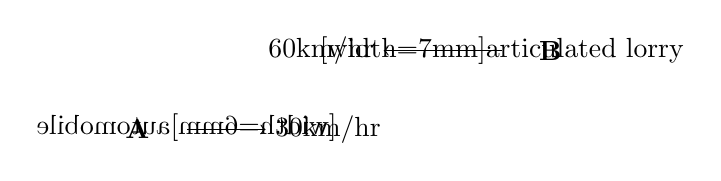
\begin{tikzpicture}
        \draw[->] (0,0) -- (1,0) node[right] {\SI{30}{km/hr}};
        \draw (0,0) node[left=1em] {\textbf{A}} node[above=-2.7mm] {\reflectbox{\twemoji[width=6mm]{automobile}}};
        \begin{scope}[xshift=4cm,yshift=1cm]
            \draw[->] (0,0) -- (-1.5,0) node[left] {\SI{60}{km/hr}};
            \draw (0,0) node[right=1em] {\textbf{B}} node[above=-3mm] {\twemoji[width=7mm]{articulated lorry}};
        \end{scope}
    \end{tikzpicture}
\end{center}

\begin{randomizechoices}
    \correctchoice \SI{-90}{km/h}
    \choice \SI{90}{km/h}
    \choice \SI{30}{km/h}
    \choice \SI{-30}{km/h}
\end{randomizechoices}

\question
What is the velocity of car B relative to the velocity of car A? Assume rightward motion is poistive; lefward motion, negative.

\begin{center}
    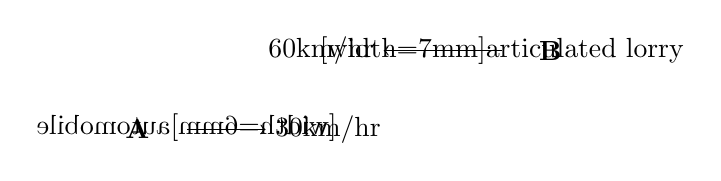
\begin{tikzpicture}
        \draw[->] (0,0) -- (1,0) node[right] {\SI{30}{km/hr}};
        \draw (0,0) node[left=1em] {\textbf{A}} node[above=-2.7mm] {\reflectbox{\twemoji[width=6mm]{automobile}}};
        \begin{scope}[xshift=4cm,yshift=1cm]
            \draw[->] (0,0) -- (-1.5,0) node[left] {\SI{60}{km/hr}};
            \draw (0,0) node[right=1em] {\textbf{B}} node[above=-3mm] {\twemoji[width=7mm]{articulated lorry}};
        \end{scope}
    \end{tikzpicture}
\end{center}

\begin{randomizechoices}
    \choice \SI{90}{km/h}
    \correctchoice \SI{90}{km/h}
    \choice \SI{30}{km/h}
    \choice \SI{-30}{km/h}
\end{randomizechoices}







\end{questions}
\end{document}
